NetFlow and \ac{IPFIX} are the two popular protocols for IP flow information
export. NetFlow \cite{rfc3954} is a network protocol designed by Cisco
Systems, which allows routers to generate and export flow records to a
designated collector. \ac{IPFIX} \cite{rfc5101} is an open standard defined by
the IETF based on NetFlow v$9$. The wide applicability of this approach is
easily seen from the pervasive use of flow records for a set of different
network analysis applications. For instance, a survey by Sperotto \textit{et
al.} \cite{sperotto:2010} gives an overview of how network flow analysis can
be used to detect intrusion attacks. In addition, a survey by Callado
\textit{et al.} \cite{callado:2009} lists behaviour analysis of Internet
backbone traffic and general anomaly detection.

Understanding intricate traffic patterns require sophisticated flow analysis
tools that can mine flow records for such a usage.  Unfortunately current
tools fail to deliver owing to their language design and simplistic filtering
methods.  We recently proposed a flow query language design
\cite{vmarinov:2009} that aims to cater to such needs.  It can process flow
records, aggregate them into groups, apply absolute or relative filters and
invoke Allen interval algebra rules \cite{fallen:1983} to merge group records.
The expressiveness of the language can be seen from \cite{vperelman:2011}
where the authors formulate flow queries to identify flow signatures of
popular applications.

Flowy \cite{kkanev:2010} was a first feature complete Python prototype of
\ac{NFQL}. Due to performance problems, it's execution engine was rewritten in
C, called Flowy 2.0 \cite{jschauer:thesis:2011}. In this paper, we introduce
\texttt{nfql}, which extends Flowy 2.0, making it more feature complete and
optimizing its execution engine with crispier algorithms.  We show that this
iteration of our work is able to scale to real-world sized traces and has
comparable execution times to contemporary flow analysis tools.

The paper is organized as follows. In Section \ref{sec:relatedwork} we survey
the current state-of-the-art of flow-processing tools and we reason how
\texttt{nfql} is different from each one of them. In Section \ref{sec:design}
we describe the flow query language by discussing each stage of the processing
pipeline. In Section \ref{sec:implementation} we provide an overview of the
\texttt{nfql} architecture and we describe the workflow of the execution
engine. A performance evaluations comparing \texttt{nfql} against contemporary
flow processing tools alongwith with a discussion on its current limitation
and future outlook is in section \ref{sec:evaluation}. We conclude the paper
in Section \ref{sec:conclusion}.

\begin{figure*}[!t]
  \subfloat{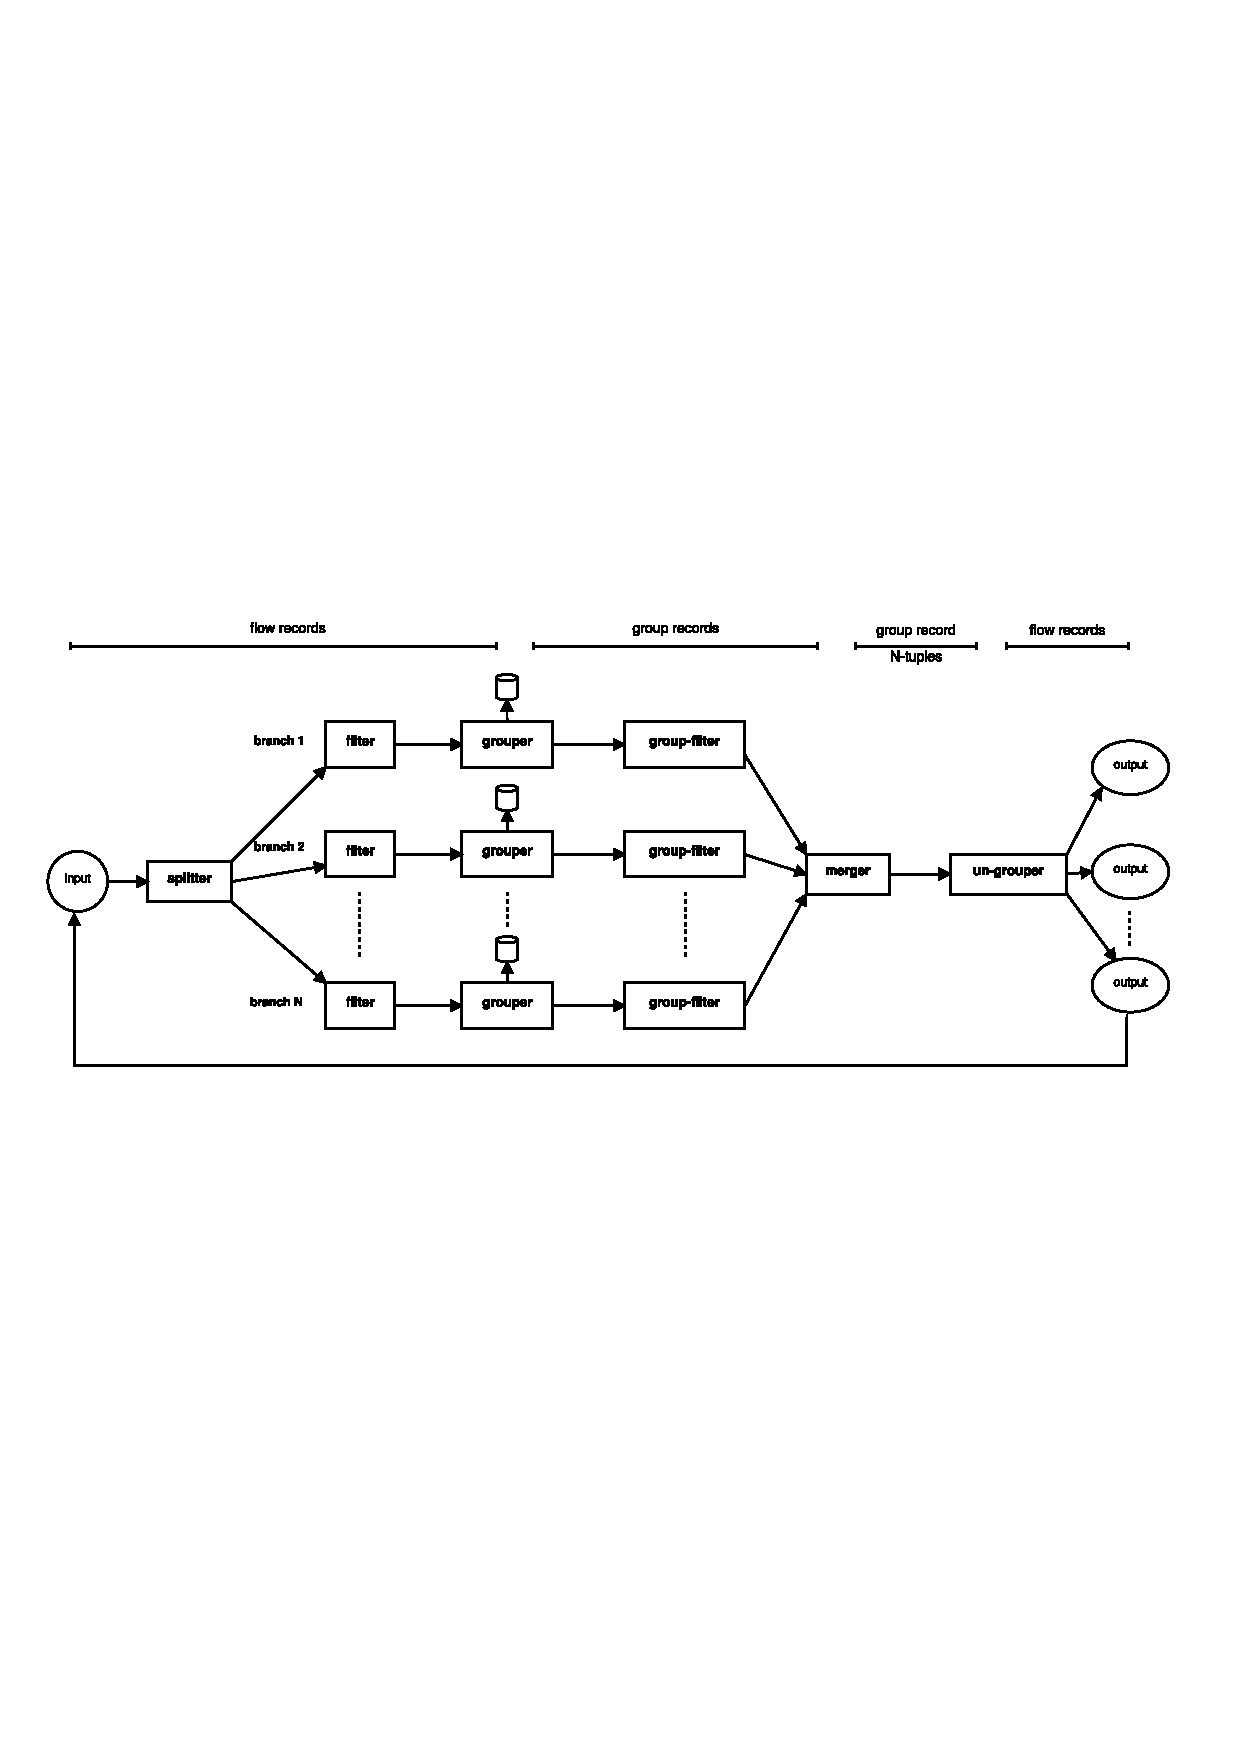
\includegraphics[width=0.7\textwidth]{nfql-pipeline}} \label{foo}
  \hfil \subfloat{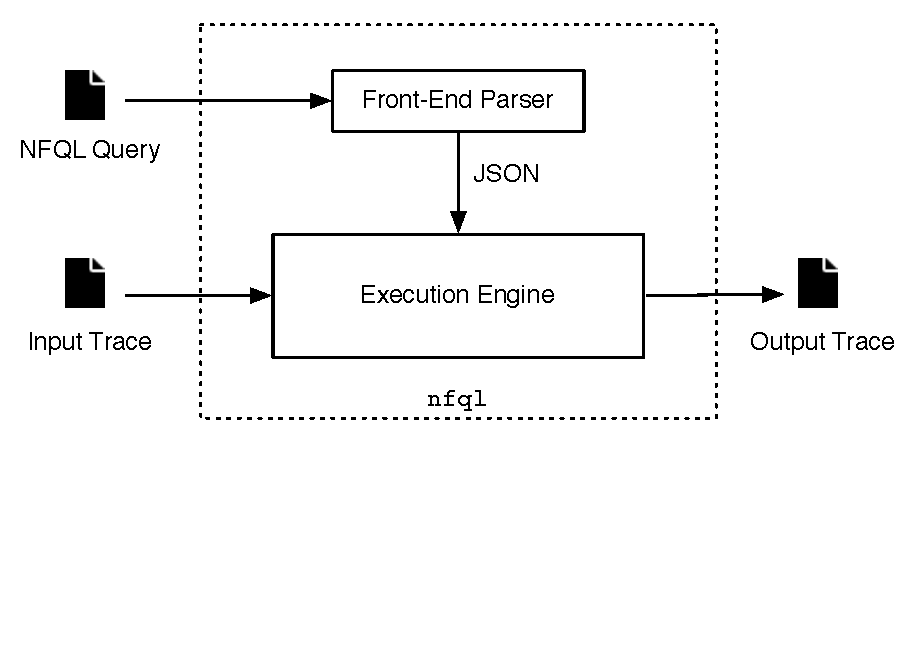
\includegraphics[width=0.3\textwidth]{nfql-architecture}}
  \label{bar} \caption{NFQL Processing Pipeline \cite{vmarinov:2009} (left)
  and \texttt{nfql} Architecture (right)} \label{fig:nfql-pipeline}
\end{figure*}
